\frame {
    \frametitle{\LARGE Выбор данных для обучения моделей}
    \vskip3.5em
    \begin{columns}
        \footnotesize
        \begin{column}{0.6\textwidth}
            Информация о выбранных наборах данных:
            \begin{itemize}
                \item 10631 снимок
                \item 27632 размеченных объекта
                \item Снимки надводных объектов с разных ракурсов как в портовой зоне, так и на открытой воде
            \end{itemize}
            
            Набор данных разбивается на обучающую, тестовую и валидационную выборки в соотношении $85:10:5$
        \end{column}

        \begin{column}{0.4\textwidth}
            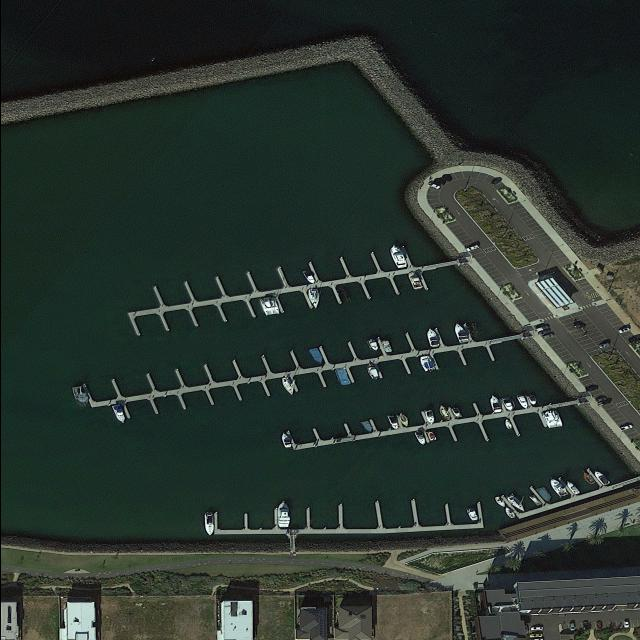
\includegraphics[scale=0.15]{inc/img/GE_17_jpg.rf.feb86f8f13e200e62e849939c5ea5c7a.jpg}
            \vskip0.5em
            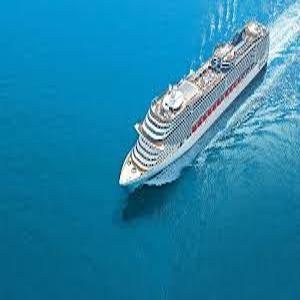
\includegraphics[scale=0.32]{inc/img/1442_jpg.rf.46c37ef66b9d0914c6e19209c278e2f5.jpg}
        \end{column}
    \end{columns}
}
